\section{Асимметричные протоколы}\label{section-protocols-asymmetric}
\selectlanguage{russian}

Асимметричные протоколы, или же протоколы, основанные на криптосистемах с открытыми ключами, позволяют ослабить требования к предварительному этапу протоколов. Вместо общего секретного ключа, который должны иметь две стороны (либо каждая из сторон и доверенный центр), в рассматриваемых ниже протоколах стороны должны предварительно обменяться открытыми ключами (между собой либо с доверенным центром). Такой предварительный обмен может проходить по открытому каналу связи, в предположении, что криптоаналитик не может повлиять на содержимое канала связи на данном этапе.

В данном разделе рассмотрены только такие протоколы, которые не описывают и не ограничивают используемые математические операции, а позволяют использовать любые надёжные криптографические примитивы из симметричной и асимметричной криптографии. При анализе надёжности таких протоколов криптостойкость используемых <<примитивных>> алгоритмов не учитывается.

\subsection{Протокол Деннинга~---~Сакко}\index{протокол!Деннинга~---~Сакко|(}
\selectlanguage{russian}

Протокол предложен Дороти Деннинг и Джованни Сакко в 1981 году (\langen{Dorothy E. Denning, Giovanni Maria Sacco},~\cite{Denning:Sacco:1981}). В данном протоколе к доверенному центру (Тренту) за сертификатами сразу обоих участников обращается инициатор (Алиса, рис.~\ref{fig:denning-sacco}). Этот же участник отвечает и за формирование нового сессионного ключа $K$.

\begin{figure}
    \centering
    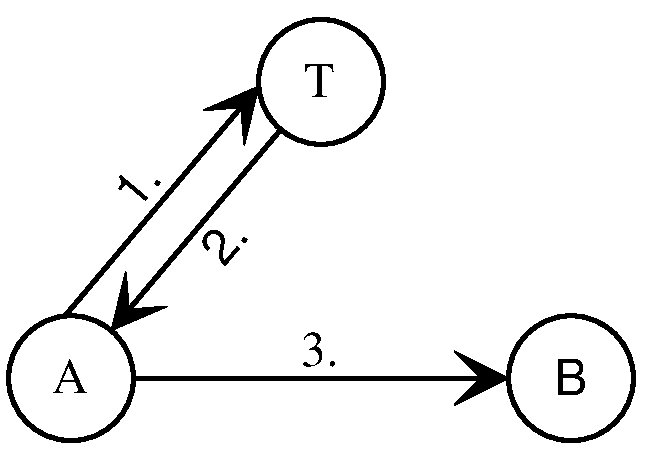
\includegraphics[width=0.5\textwidth]{pic/denning-sacco}
    \caption{Взаимодействие участников в протоколе Деннинга~---~Сакко\label{fig:denning-sacco}}
\end{figure}

\begin{protocol}
    \item[(1)] $Alice \to \left\{ A, B \right\} \to Trent$
    \item[(2)] $Trent \to \left\{ S_T( A, K_A, T_T ), S_T( B, K_B, T_T ) \right\} \to Alice$
	\item[(3)] Алиса генерирует новый сессионный ключ $K$
	\item[{}] $\begin{array}{lll}
Alice \to \{ & E_B( S_A ( K, T_A ) ), & \\ 
             & S_T( A, K_A, T_T ),    & \\ 
             & S_T( B, K_B, T_T )     & \} \to Bob
\end{array}$
	\item[(4)] Боб проверяет подпись доверенного центра на сертификате $S_T( A, K_A, T_T )$, расшифровывает сессионный ключ $K$ и проверяет подпись Алисы.
\end{protocol}

Отсутствие в сообщении $E_B( S_A ( K, T_A ) )$ каких-либо идентификаторов делает протокол уязвимым к атаке с известными сеансовым ключом\index{атака!с известным разовым ключом} и позволяет второй стороне (Бобу) выдать себя за инициатора (Алису) в сеансе с третьей стороной (Кларой, рис.~\ref{fig:denning-sacco-attack}).

\begin{figure}
    \centering
    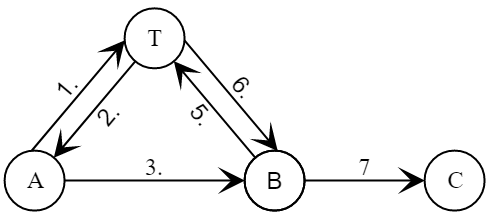
\includegraphics[width=0.67\textwidth]{pic/denning-sacco-attack}
    \caption{Взаимодействие участников в протоколе Деннинга~---~Сакко\label{fig:denning-sacco-attack}}
\end{figure}

\begin{protocol}
    \item[(1)--(4)] Алиса и Боб провели сеанс протокола, выработав новый сессионный ключ $K$.
    \item[(5)] $Bob \to \left\{ B, C \right\} \to Trent$
    \item[(6)] $Trent \to \left\{ S_T( B, K_B, T_T ), S_T( C, K_C, T_T ) \right\} \to Bob$
	\item[(7)] Боб воспроизводит сообщения $S_A ( K, T_A )$ и $S_T( A, K_A, T_T )$ от Алисы в сеансе с Кларой:
    \item[{}] $\begin{array}{lll}
Bob~(Alice) \to \{ & E_C( S_A ( K, T_A ) ), & \\ 
             & S_T( A, K_A, T_T ),    & \\ 
             & S_T( C, K_C, T_T )     & \} \to Clara
\end{array}$
	\item[(8)] Клара успешно проверяет подпись доверенного центра на сертификате $S_T( A, K_A, T_T )$, расшифровывает сессионный ключ $K$ и проверяет подпись Алисы.
\end{protocol}

В результате Клара уверена, что получила от Алисы новый сессионный ключ $K$.

\index{протокол!Деннинга~---~Сакко|)}

\subsection{Протокол DASS}\index{протокол!DASS|(}
\selectlanguage{russian}

Протокол DASS являлся составной частью сервиса распределённой аутентификации DASS (\langen{Distributed Authentication Security Service}), разработанного компанией DEC и описанного в RFC 1507~\cite{rfc1507} в сентябре 1993 года.

В протоколе DASS, по аналогии с протоколами Wide-Mouth Frog и Деннинга~---~Сакко, инициатор (Алиса) генерирует и новый сеансовый ключ, и, для каждого сеанса протокола, новую пару открытого и закрытого ключей отправителя. Доверенный центр (Трент) используется как хранилище сертификатов открытых ключей участников. Но в отличие от Деннинга~---~Сакко к доверенному центру обращаются по очереди оба участника.

\begin{figure}
    \centering
    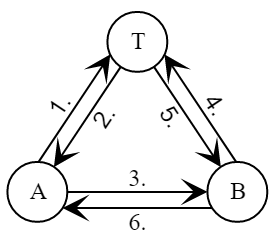
\includegraphics[width=0.5\textwidth]{pic/key_distribution-dass}
    \caption{Взаимодействие участников в протоколе DASS\label{fig:key_distribution-dass}}
\end{figure}

\begin{protocol}
    \item[(1)] $Alice \to \left\{ B \right\} \to Trent$
    \item[(2)] $Trent \to \left\{ S_T \left( B, K_B \right) \right\} \to Alice$
    \item[(3)] $Alice \to \left\{ E_K \left( T_A \right), S_A \left( L, A, K_P \right), S_{K_P} \left( E_B \left( K \right) \right) \right\} \to Bob$
    \item[(4)] $Bob \to \left\{ A \right\} \to Trent$
    \item[(5)] $Trent \to \left\{ S_T \left( A, K_A \right) \right\} \to Bob$
    \item[(6)] $Bob \to \left\{ E_K \left\{ T_B \right\} \right\} \to Alice$
\end{protocol}

С помощью сертификатов открытых ключей $\left\{ S_T \left( B, K_B \right) \right\}$ и $\left\{ S_T \left( A, K_A \right) \right\}$, которые отправляет Трент, и дальнейшего подтверждения владения соответствующими ключами, участники могут аутентифицировать друг-друга. Успешная расшифровка временных меток из сообщений $E_K \left( T_A \right)$ и $E_K \left\{ T_B \right\}$ обеспечивает подтверждение владением сеансовым ключом.

В протоколе используется время жизни ($L$) сеансового ключа $K_P$, однако в сообщение не включена метка времени. В результате протокол остаётся уязвимым к атаке с известным сеансовым ключом. Предположим, что Меллори смогла записать полностью прошедший сеанс связи между Алисой и Бобом, а потом смогла получить доступ к сеансовому ключу $K$. Это позволяет Меллори аутентифицировать себя как Алиса перед Бобом.

\begin{protocol}
    \item[(1)] $Mellory~(Alice) \to \left\{ E_K \left( T_M \right), S_A \left( L, A, K_P \right), S_{K_P} \left( E_B \left( K \right) \right) \right\} \to Bob$
    \item[(2)] $Bob \to \left\{ A \right\} \to Trent$
    \item[(3)] $Trent \to \left\{ S_T \left( A, K_A \right) \right\} \to Bob$
    \item[(4)] $Bob \to \left\{ E_K \left\{ T_B \right\} \right\} \to Alice$
\end{protocol}

На первом проходе Меллори меняет только первое сообщение, содержащее метку времени $E_K \left( T_M \right)$. Всё остальное Меллори копирует из записанного сеанса связи. Если Боб не записывает используемые ключи, он не заметит подмены. Простейшее исправление данной уязвимости состоит во включении метки времени в сообщение $S_A \left( T_A, L, A, K_P \right)$.

Так как в протоколе сеансовый ключ $K$ шифруется <<мастер>>-ключом Боба $K_B$, то компрометация последнего приведёт к компрметации всех использованных ранее сеансовых ключей. То есть протокол не обеспечивает совершенной прямой секретности (цель G9).

Ни Трент, ни Боб не участвуют в формировании новых сеансовых ключей. Поэтому Алиса может заставить Боба использовать старый сеансовый ключ, как в протоколах Wide-Mouth Frog\index{протокол!Wide-Mouth Frog} и Yahalom\index{протокол!Yahalom}.

\index{протокол!DASS|)}

\subsection{Протокол Ву~---~Лама}\index{протокол!Ву~---~Лама|(}\label{section-woo-lam}
\selectlanguage{russian}

Протокол Ву~---~Лама, предложенный в 1992 году (\langen{Woo, Lam},~\cite{Woo:Lam:1992:1, Woo:Lam:1992:3}), добавляет к сообщениям случайные числа участников, что позволяет защитить протокол в том числе от атак повтором, а также обеспечивает подтверждение владения ключами. Также это единственный из рассмотренных в этом разделе протоколов, в котором новый ключ формируется доверенной стороной (Трентом).

\begin{figure}
    \centering
    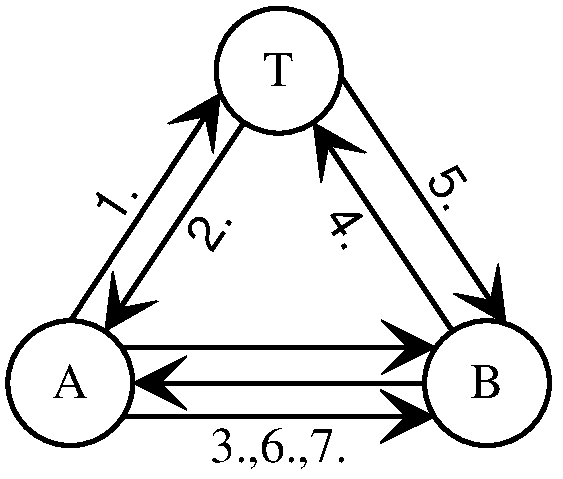
\includegraphics[width=0.5\textwidth]{pic/woo-lam}
    \caption{Взаимодействие участников в протоколе Ву~---~Лама\label{fig:woo-lam}}
\end{figure}

\begin{protocol}
    \item[(1)] $Alice \to \left\{ A, B \right\} \to Trent$
    \item[(2)] $Trent \to \left\{ S_T( K_B ) \right\} \to Alice$
    \item[(3)] $Alice \to \left\{ E_B ( A, R_A ) \right\} \to Bob$
    \item[(4)] $Bob \to \left\{ A, B, E_T( R_A ) \right\} \to Trent$
    \item[(5)] $Trent \to \left\{ S_T( K_A ), E_B ( S_T ( R_A, K, A, B ) ) \right\} \to Bob$
    \item[(6)] $Bob \to \left\{ E_A (S_T (R_A, K, A, B), R_B) \right\} \to Alice$
    \item[(7)] $Alice \to \left\{ E_K( R_B ) \right\} \to Bob$
\end{protocol}

Так как в сертификате сессионного ключа $S_T (R_A, K, A, B)$ присутствует случайное число Алисы $R_A$, то злоумышленник не сможет использовать старый сертификат в новом сеансе от имени Боба. Следовательно 6-й проход протокола позволяет Алисе убедиться, что Боб знает новый сессионный ключ $K$, и, следовательно владеет своим <<мастер>>-ключом $K_B$ (так как это единственный способ получить сертификат из сообщения $E_B ( S_T ( R_A, K, A, B ) ))$).

Сообщение $E_K( R_B )$ от Алисы к Бобу на седьмом проходе позволяет одновременно гарантировать, что Алиса знает и свой <<мастер>>-ключ $K_A$ (так как смогла расшифровать $E_A(\dots, R_B)$), и новый сессионный ключ $K$, так как смогла корректно зашифровать $R_B$ этим ключом.

\index{протокол!Ву~---~Лама|)}
